\documentclass[twoside]{book}

% Packages required by doxygen
\usepackage{fixltx2e}
\usepackage{calc}
\usepackage{doxygen}
\usepackage[export]{adjustbox} % also loads graphicx
\usepackage{graphicx}
\usepackage[utf8]{inputenc}
\usepackage{makeidx}
\usepackage{multicol}
\usepackage{multirow}
\PassOptionsToPackage{warn}{textcomp}
\usepackage{textcomp}
\usepackage[nointegrals]{wasysym}
\usepackage[table]{xcolor}

% Font selection
\usepackage[T1]{fontenc}
\usepackage[scaled=.90]{helvet}
\usepackage{courier}
\usepackage{amssymb}
\usepackage{sectsty}
\renewcommand{\familydefault}{\sfdefault}
\allsectionsfont{%
  \fontseries{bc}\selectfont%
  \color{darkgray}%
}
\renewcommand{\DoxyLabelFont}{%
  \fontseries{bc}\selectfont%
  \color{darkgray}%
}
\newcommand{\+}{\discretionary{\mbox{\scriptsize$\hookleftarrow$}}{}{}}

% Page & text layout
\usepackage{geometry}
\geometry{%
  a4paper,%
  top=2.5cm,%
  bottom=2.5cm,%
  left=2.5cm,%
  right=2.5cm%
}
\tolerance=750
\hfuzz=15pt
\hbadness=750
\setlength{\emergencystretch}{15pt}
\setlength{\parindent}{0cm}
\setlength{\parskip}{3ex plus 2ex minus 2ex}
\makeatletter
\renewcommand{\paragraph}{%
  \@startsection{paragraph}{4}{0ex}{-1.0ex}{1.0ex}{%
    \normalfont\normalsize\bfseries\SS@parafont%
  }%
}
\renewcommand{\subparagraph}{%
  \@startsection{subparagraph}{5}{0ex}{-1.0ex}{1.0ex}{%
    \normalfont\normalsize\bfseries\SS@subparafont%
  }%
}
\makeatother

% Headers & footers
\usepackage{fancyhdr}
\pagestyle{fancyplain}
\fancyhead[LE]{\fancyplain{}{\bfseries\thepage}}
\fancyhead[CE]{\fancyplain{}{}}
\fancyhead[RE]{\fancyplain{}{\bfseries\leftmark}}
\fancyhead[LO]{\fancyplain{}{\bfseries\rightmark}}
\fancyhead[CO]{\fancyplain{}{}}
\fancyhead[RO]{\fancyplain{}{\bfseries\thepage}}
\fancyfoot[LE]{\fancyplain{}{}}
\fancyfoot[CE]{\fancyplain{}{}}
\fancyfoot[RE]{\fancyplain{}{\bfseries\scriptsize Generated by Doxygen }}
\fancyfoot[LO]{\fancyplain{}{\bfseries\scriptsize Generated by Doxygen }}
\fancyfoot[CO]{\fancyplain{}{}}
\fancyfoot[RO]{\fancyplain{}{}}
\renewcommand{\footrulewidth}{0.4pt}
\renewcommand{\chaptermark}[1]{%
  \markboth{#1}{}%
}
\renewcommand{\sectionmark}[1]{%
  \markright{\thesection\ #1}%
}

% Indices & bibliography
\usepackage{natbib}
\usepackage[titles]{tocloft}
\setcounter{tocdepth}{3}
\setcounter{secnumdepth}{5}
\makeindex

% Hyperlinks (required, but should be loaded last)
\usepackage{ifpdf}
\ifpdf
  \usepackage[pdftex,pagebackref=true]{hyperref}
\else
  \usepackage[ps2pdf,pagebackref=true]{hyperref}
\fi
\hypersetup{%
  colorlinks=true,%
  linkcolor=blue,%
  citecolor=blue,%
  unicode%
}

% Custom commands
\newcommand{\clearemptydoublepage}{%
  \newpage{\pagestyle{empty}\cleardoublepage}%
}

\usepackage{caption}
\captionsetup{labelsep=space,justification=centering,font={bf},singlelinecheck=off,skip=4pt,position=top}

%===== C O N T E N T S =====

\begin{document}

% Titlepage & ToC
\hypersetup{pageanchor=false,
             bookmarksnumbered=true,
             pdfencoding=unicode
            }
\pagenumbering{alph}
\begin{titlepage}
\vspace*{7cm}
\begin{center}%
{\Large V\+E\+R\+S\+EM }\\
\vspace*{1cm}
{\large Generated by Doxygen 1.8.14}\\
\end{center}
\end{titlepage}
\clearemptydoublepage
\pagenumbering{roman}
\tableofcontents
\clearemptydoublepage
\pagenumbering{arabic}
\hypersetup{pageanchor=true}

%--- Begin generated contents ---
\chapter{V\+E\+R\+S\+EM}
\label{md__r_e_a_d_m_e}
\Hypertarget{md__r_e_a_d_m_e}
Initial, empty R\+E\+A\+D\+ME for the V\+E\+Rsatile Spectral Element Method. 
\chapter{Hierarchical Index}
\section{Class Hierarchy}
This inheritance list is sorted roughly, but not completely, alphabetically\+:\begin{DoxyCompactList}
\item Test\+Case\begin{DoxyCompactList}
\item \contentsline{section}{test\+\_\+gll.\+Test\+G\+LL}{\pageref{classtest__gll_1_1_test_g_l_l}}{}
\end{DoxyCompactList}
\end{DoxyCompactList}

\chapter{Class Index}
\section{Class List}
Here are the classes, structs, unions and interfaces with brief descriptions\+:\begin{DoxyCompactList}
\item\contentsline{section}{\mbox{\hyperlink{classtest__gll_1_1_test_g_l_l}{test\+\_\+gll.\+Test\+G\+LL}} }{\pageref{classtest__gll_1_1_test_g_l_l}}{}
\end{DoxyCompactList}

\chapter{Class Documentation}
\hypertarget{classtest__gll_1_1_test_g_l_l}{}\section{test\+\_\+gll.\+Test\+G\+LL Class Reference}
\label{classtest__gll_1_1_test_g_l_l}\index{test\+\_\+gll.\+Test\+G\+LL@{test\+\_\+gll.\+Test\+G\+LL}}
Inheritance diagram for test\+\_\+gll.\+Test\+G\+LL\+:\begin{figure}[H]
\begin{center}
\leavevmode
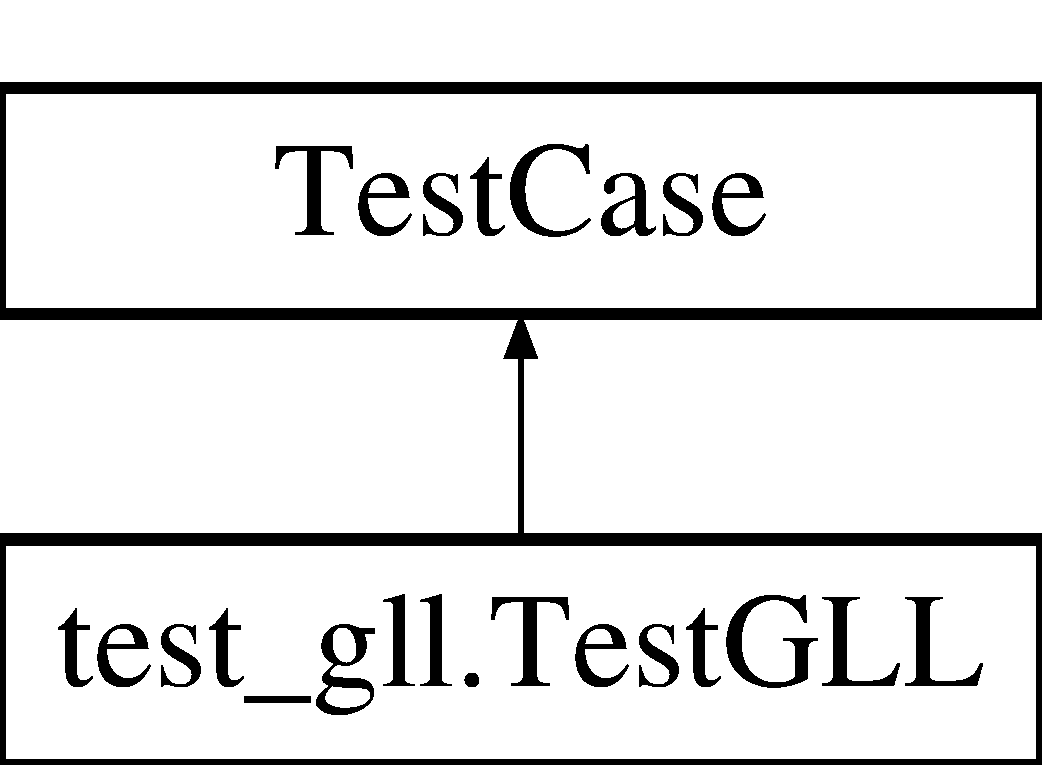
\includegraphics[height=2.000000cm]{classtest__gll_1_1_test_g_l_l}
\end{center}
\end{figure}
\subsection*{Public Member Functions}
\begin{DoxyCompactItemize}
\item 
def \mbox{\hyperlink{classtest__gll_1_1_test_g_l_l_a1357eaab2f6d378ac53e9ae0276d2a2b}{test\+G\+L\+L\+Points\+And\+Weights2}} (self)
\item 
def \mbox{\hyperlink{classtest__gll_1_1_test_g_l_l_a95fd324973c22c9edae81c4adbed0c4f}{test\+Lagrange\+Poly}} (self)
\end{DoxyCompactItemize}


\subsection{Detailed Description}
\begin{DoxyVerb}Testing functions of the gll_library 
- Gauss-Lobatto-Legendre points and weights
- Lagrange Polynomial evaluator\end{DoxyVerb}
 

\subsection{Member Function Documentation}
\mbox{\Hypertarget{classtest__gll_1_1_test_g_l_l_a1357eaab2f6d378ac53e9ae0276d2a2b}\label{classtest__gll_1_1_test_g_l_l_a1357eaab2f6d378ac53e9ae0276d2a2b}} 
\index{test\+\_\+gll\+::\+Test\+G\+LL@{test\+\_\+gll\+::\+Test\+G\+LL}!test\+G\+L\+L\+Points\+And\+Weights2@{test\+G\+L\+L\+Points\+And\+Weights2}}
\index{test\+G\+L\+L\+Points\+And\+Weights2@{test\+G\+L\+L\+Points\+And\+Weights2}!test\+\_\+gll\+::\+Test\+G\+LL@{test\+\_\+gll\+::\+Test\+G\+LL}}
\subsubsection{\texorpdfstring{test\+G\+L\+L\+Points\+And\+Weights2()}{testGLLPointsAndWeights2()}}
{\footnotesize\ttfamily def test\+\_\+gll.\+Test\+G\+L\+L.\+test\+G\+L\+L\+Points\+And\+Weights2 (\begin{DoxyParamCaption}\item[{}]{self }\end{DoxyParamCaption})}

\begin{DoxyVerb}Tests gll_pw() from gll_library whether points and weights 
are correct. Note that it is almost equal due to the fact that
the points are hardcoded.
\end{DoxyVerb}
 \mbox{\Hypertarget{classtest__gll_1_1_test_g_l_l_a95fd324973c22c9edae81c4adbed0c4f}\label{classtest__gll_1_1_test_g_l_l_a95fd324973c22c9edae81c4adbed0c4f}} 
\index{test\+\_\+gll\+::\+Test\+G\+LL@{test\+\_\+gll\+::\+Test\+G\+LL}!test\+Lagrange\+Poly@{test\+Lagrange\+Poly}}
\index{test\+Lagrange\+Poly@{test\+Lagrange\+Poly}!test\+\_\+gll\+::\+Test\+G\+LL@{test\+\_\+gll\+::\+Test\+G\+LL}}
\subsubsection{\texorpdfstring{test\+Lagrange\+Poly()}{testLagrangePoly()}}
{\footnotesize\ttfamily def test\+\_\+gll.\+Test\+G\+L\+L.\+test\+Lagrange\+Poly (\begin{DoxyParamCaption}\item[{}]{self }\end{DoxyParamCaption})}

\begin{DoxyVerb}Tests lagrange() from the gll_library\end{DoxyVerb}
 

The documentation for this class was generated from the following file\+:\begin{DoxyCompactItemize}
\item 
tests/test\+\_\+gll.\+py\end{DoxyCompactItemize}

%--- End generated contents ---

% Index
\backmatter
\newpage
\phantomsection
\clearemptydoublepage
\addcontentsline{toc}{chapter}{Index}
\printindex

\end{document}
